\documentclass[
11pt, % The default document font size, options: 10pt, 11pt, 12pt
%codirector, % Uncomment to add a codirector to the title page
]{charter} 
\usepackage[utf8]{inputenc}   % Paquete para codificación
\usepackage[T1]{fontenc}      % Paquete para fuentes
\usepackage[spanish]{babel}   % Paquete para idioma español
\usepackage{graphicx}         % Para imágenes
\usepackage{tabularx}    
\usepackage{xcolor}   
\usepackage{pdflscape}

\usepackage{geometry}
\usepackage{xcolor}
\usepackage{caption}  



% El títulos de la memoria, se usa en la carátula y se puede usar el cualquier lugar del documento con el comando \ttitle
\titulo{Modernización de contadores de tránsito con comunicación bidireccional} 

% Nombre del posgrado, se usa en la carátula y se puede usar el cualquier lugar del documento con el comando \degreename
%\posgrado{Carrera de Especialización en Sistemas Embebidos} 
\posgrado{Carrera de Especialización en Internet de las Cosas} 
%\posgrado{Carrera de Especialización en Inteligencia Artificial}
%\posgrado{Maestría en Sistemas Embebidos} 
%\posgrado{Maestría en Internet de las cosas}

% Tu nombre, se puede usar el cualquier lugar del documento con el comando \authorname
% IMPORTANTE: no omitir titulaciones ni tildación en los nombres, también se recomienda escribir los nombres completos (tal cual los tienen en su documento)
\autor{Ing. Diego Aníbal Vázquez}

% El nombre del director y co-director, se puede usar el cualquier lugar del documento con el comando \supname y \cosupname y \pertesupname y \pertecosupname
\director{-}
\pertenenciaDirector{-} 
\codirector{} % para que aparezca en la portada se debe descomentar la opción codirector en los parámetros de documentclass
\pertenenciaCoDirector{FIUBA}

% Nombre del cliente, quien va a aprobar los resultados del proyecto, se puede usar con el comando \clientename y \empclientename
\cliente{Subgerencia de Estudios de Demanda}
\empresaCliente{Vialidad Nacional}
 
\fechaINICIO{29 de abril de 2025}		%Fecha de inicio de la cursada de GdP \fechaInicioName
\fechaFINALPlan{17 de junio de 2025} 	%Fecha de final de cursada de GdP
\fechaFINALTrabajo{marzo de 2026}	%Fecha de defensa pública del trabajo final


\begin{document}

\maketitle
\thispagestyle{empty}
\pagebreak


\thispagestyle{empty}
{\setlength{\parskip}{0pt}
\tableofcontents{}
}
\pagebreak


\section*{Registros de cambios}
\label{sec:registro}


\begin{table}[ht]
\label{tab:registro}
\centering
\begin{tabularx}{\linewidth}{@{}|c|X|c|@{}}
\hline
\rowcolor[HTML]{C0C0C0} 
Revisión & \multicolumn{1}{c|}{\cellcolor[HTML]{C0C0C0}Detalles de los cambios realizados} & Fecha      \\ \hline
0      & Creación del documento                                 &\fechaInicioName \\ \hline
1      & Se completa hasta el punto 5 inclusive                & {13} de {mayo} de 2025 \\ \hline
2      & Se completa hasta el punto 9 inclusive        & {20} de {mayo} de 2025 \\
\hline
%		  Se puede agregar algo más \newline
%		  En distintas líneas \newline
%		  Así                                                    & {día} de {mes} de 202X \\ %3      & Se completa hasta el punto 12 inclusive                & {día} de {mes} de 202X \\ \hline
%4      & Se completa el plan	                                 & {día} de {mes} de 202X \\ \hline

% Si hay más correcciones pasada la versión 4 también se deben especificar acá

\end{tabularx}
\end{table}

\pagebreak



\section*{Acta de constitución del proyecto}
\label{sec:acta}

\begin{flushright}
Buenos Aires, \fechaInicioName
\end{flushright}

\vspace{2cm}
Por medio de la presente se acuerda con el \authorname\hspace{1px} que su Trabajo Final de la \degreename\hspace{1px} se titulará ``\ttitle'' y consistirá en {un sistema de comunicación con los contadores de tránsito, que incorpore un modelo bidireccional. El trabajo tendrá un presupuesto preliminar estimado de 600} horas y un costo estimado de \$ - , con fecha de inicio el \fechaInicioName\hspace{1px} y fecha de presentación pública el \fechaFinalName.
Se adjunta a esta acta la planificación inicial.
\vfill
% Esta parte se construye sola con la información que hayan cargado en el preámbulo del documento y no debe modificarla
\begin{table}[ht]
\centering
\begin{tabular}{ccc}
\begin{tabular}[c]{@{}c@{}}Dr. Ing. Ariel Lutenberg \\ Director posgrado FIUBA\end{tabular} & \hspace{2cm} & \begin{tabular}[c]{@{}c@{}}\clientename \\ \empclientename \end{tabular} \vspace{2.5cm} \\ 
\multicolumn{3}{c}{\begin{tabular}[c]{@{}c@{}} \supname \\ Director del Trabajo Final\end{tabular}} \vspace{2.5cm} \\
\end{tabular}
\end{table}

\section{1. Descripción técnica-conceptual del proyecto a realizar}
\label{sec:descripcion}

%\begin{consigna}{red} % ELIMINAR \begin{consigna}{red} y \end{consigna}{red} en las secciones que vayan completando para cada entrega parcial.


\subsection{Contexto y motivación}
Este proyecto surge a partir de una necesidad detectada en la infraestructura actual de monitoreo del tránsito vehicular utilizada en rutas nacionales.

Actualmente, uno de los modelos de contadores de tránsito empleados ha sido desarrollado internamente y cumple adecuadamente su función básica: registrar el paso de vehículos, clasificarlos por carril en livianos y pesados y transmitir los datos a un servidor central.

Sin embargo, estas unidades se comunican exclusivamente mediante enlaces GPRS tercerizados a través de un canal unidireccional. Esto impide cualquier tipo de interacción remota con los dispositivos en campo.

Frente a esta situación, se plantea el desafío de modernizar la arquitectura de comunicaciones del sistema, incorporando capacidades de comunicación bidireccional, diagnóstico remoto y respuesta operativa rápida.

\subsection{Problemas identificados}

\begin{itemize}

\item Falta de comunicación bidireccional: actualmente, no es posible enviar comandos desde el servidor a los dispositivos para ajustar su configuración, reiniciarlos o recolectar información de diagnóstico.

\item Dependencia de proveedores externos: la infraestructura GPRS utilizada es tercerizada, lo que genera costos recurrentes, posibles restricciones técnicas y dificultades para gestionar incidentes de manera eficiente.

\item Imposibilidad de actualización remota: cualquier modificación de parámetros de funcionamiento requiere intervención física en el dispositivo, lo que limita la flexibilidad y agilidad operativa.

\end{itemize}

\subsection{Estado del arte y propuesta de valor}
En el mercado existen diversas soluciones comerciales que ofrecen capacidades de gestión remota y comunicación bidireccional. Sin embargo, muchas de ellas resultan costosas.

El enfoque propuesto busca aprovechar tecnologías de código abierto y protocolos estandarizados (MQTT), con el objetivo de construir una alternativa flexible, escalable y económicamente viable adaptada al entorno específico de las rutas argentinas.
\subsection{Propuesta de modernización}

Se propone rediseñar el sistema de comunicaciones de los contadores de tránsito mediante la incorporación de un modelo de comunicación bidireccional y segura.
Este nuevo esquema permitirá no solo el envío de datos desde los dispositivos hacia el servidor central, sino también la recepción de comandos y actualizaciones de parámetros desde el servidor hacia los dispositivos en el campo.
Además se prevé la visualización de los datos en tiempo real conforme se transmiten.

\subsection{Descripción funcional y técnica}

El sistema estará compuesto por un dispositivo contador con capacidad de comunicación bidireccional mediante GPRS, utilizando el protocolo MQTT para el envío seguro de datos. La información capturada será almacenada en una base de datos relacional y visualizada a través de una interfaz web básica alojada en el servidor central. Esta interfaz permitirá el monitoreo en tiempo real así como el envío de comandos remotos. Además, se incluirán funciones de monitoreo de temperatura, nivel de batería y detección de errores de hardware o comunicación.




\subsection{Grado de innovación}
La innovación del proyecto radica en la integración de elementos existentes , como sensores y redes móviles, bajo una arquitectura abierta y centralizada, adaptable y orientada a la gestión inteligente de los datos de tránsito, con un fuerte énfasis en la autonomía y flexibilidad operativa.


En la figura \ref{fig:diagBloques} se presenta el diagrama en bloques del sistema. El dispositivo de conteo, compuesto por sensores y un microcontrolador, se comunica mediante un canal inalámbrico GPRS y transmite los datos hacia un broker MQTT externo. El servidor central está suscrito a este broker y recibe los datos mediante un módulo de procesamiento que los almacena en una base de datos relacional. Paralelamente, el sistema cuenta con una API REST que permite el acceso a la información desde una interfaz web y la ejecución de comandos administrativos. De esta manera, el sistema combina la eficiencia del protocolo MQTT para el envío de datos en tiempo real con la flexibilidad de una API REST para la gestión y visualización.

\begin{figure}[htpb]
\centering 
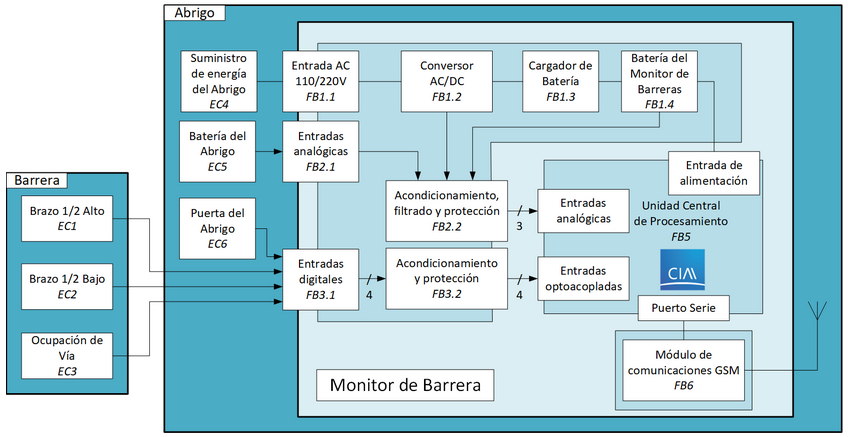
\includegraphics[width=.90\textwidth]{./Figuras/diagBloques.png}
\caption{Diagrama en bloques del sistema.}
\label{fig:diagBloques}
\end{figure}

\vspace{25px}


\section{2. Identificación y análisis de los interesados}
\label{sec:interesados}



\begin{table}[h!]
\renewcommand{\arraystretch}{1.4} % Aumenta el espacio entre filas
\centering
\begin{tabular}{|p{3cm}|p{4.5cm}|p{4.5cm}|p{4.5cm}|}
\hline
\textbf{Rol} & \textbf{Nombre y apellido} & \textbf{Organización} & \textbf{Puesto} \\
\hline
Auspiciante   & \empclientename             & -                & -                                \\
\hline
Cliente       & \clientename                & \empclientename  & -                                \\
\hline
Impulsor      & Ing. Rogelio Diego González & \empclientename  & Subgerente de Estudios de Demanda \\
\hline
Responsable   & \authorname                 & FIUBA            & Alumno                           \\
\hline
Colaboradora  & Ing. María Clara Cutrone    & \empclientename  & Jefa Sección Análisis Tránsito   \\
\hline
Colaborador   & Ing. Alejandro Di Rosso     & \empclientename  & Jefe Sección Censos de Carga     \\
\hline
Orientador    & \supname                    & \pertesupname    & Director del Trabajo Final       \\
\hline
Opositores    & ATSA                        & -                & -                                \\
\hline
Usuario final & \clientename                & \empclientename  & -                                \\
\hline
Usuario final & Gerencia Ejecutiva de Proyectos y Obras & \empclientename & -             \\
\hline
Usuario final & Consultoras Externas        & -                & -                                \\
\hline
\end{tabular}
\caption{Identificación de los interesados}
\label{tab:interesados}
\end{table}



\begin{table}[h!]
\renewcommand{\arraystretch}{1.4} % Aumenta el espacio entre filas
\centering
\begin{tabular}{|p{3cm}|p{4.5cm}|p{8cm}|}
\hline
\textbf{Rol} & \textbf{Nombre y apellido} & \textbf{Observaciones} \\
\hline
Auspiciante & \empclientename & Es exigente con la rendición de gastos. Se deberá tener especial cuidado en este aspecto. \\
\hline
Cliente & \clientename & Valora especialmente la autonomía operativa, la posibilidad de diagnóstico remoto y la reducción de costos operativos. No hay condiciones especiales relacionadas con la propiedad intelectual ni con la confidencialidad. \\
\hline
Colaboradora & Ing. María Clara Cutrone & Suele pedir licencia debido a una familia extensa. La planificación debe considerar esta situación. \\
\hline
\end{tabular}
\caption{Participantes y consideraciones relevantes}
\end{table}




\section{3. Propósito del proyecto}
\label{sec:proposito}

Diseñar e implementar un sistema capaz de registrar eventos de tránsito y permitir la transmisión segura de los datos recolectados, incluso ante cortes de conexión. Además, se busca incorporar capacidades de comunicación bidireccional que habiliten diagnósticos remotos y la carga de actualizaciones de parámetros, así como una mejor respuesta ante fallas. Con ello, se pretende mejorar la calidad de la información recolectada en rutas nacionales y facilitar el trabajo de los equipos técnicos responsables del monitoreo.

\section{4. Alcance del proyecto}
\label{sec:alcance}


Se desarrollará un prototipo funcional que permita validar los aspectos clave del rediseño propuesto.
El prototipo incluirá:

\begin{itemize}
	\item Un dispositivo contador actualmente existente, pero incompleto, al que se le incorporará la capacidad de comunicación bidireccional.
	\item Un canal de comunicación GPRS.
	\item Implementación de un protocolo seguro (MQTT) para el envío y recepción de datos y comandos.
	\item Una interfaz básica en el servidor central para la visualización de datos en tiempo real y el envío de instrucciones al dispositivo.
	\item Funciones elementales de monitoreo remoto.
	\item Base de datos relacional en el servidor central para el almacenamiento estructurado de los datos recibidos desde los dispositivos de campo.
	
\end{itemize}

El presente proyecto no incluye el desarrollo ni la implementación de algoritmos de inteligencia artificial para estimar o reconstruir tránsitos no detectados.

\section{5. Supuestos del proyecto}
\label{sec:supuestos}

Para el desarrollo del presente proyecto se supone que:

\begin{itemize}
	\item Se dispone de acceso a la infraestructura actual de los contadores de tránsito ya instalados, así como de la documentación técnica necesaria para su análisis y eventual integración.
	\item Se cuenta con conectividad intermitente por GPRS en los sitios donde se instalará el sistema, lo que permitirá validar el funcionamiento del envío diferido de datos.
	\item Los recursos humanos involucrados  estarán disponibles durante la duración del proyecto en los tiempos y roles previstos.
	\item Los materiales requeridos (hardware de prueba, sensores, dispositivos de comunicación, etc.), estarán disponibles o serán reemplazables por equivalentes funcionales en caso de faltantes.
	\item La incorporación de comunicación bidireccional es técnicamente factible y puede realizarse sin rediseñar completamente el hardware existente.
\end{itemize}

\section{6. Requerimientos}
\label{sec:requerimientos}


\begin{enumerate}
	\item \textbf{Requerimientos funcionales:}
			\begin{enumerate}
			\item El ESP32-C3 debe recibir datos por interfaz \textbf{RS-232} desde el sistema de detección.
			\item  Cada evento recibido debe ser \textbf{encolado en memoria RAM} en el orden de llegada.
			\item  El ESP32-C3 debe publicar cada mensaje de la cola a un \textbf{broker MQTT} remoto usando GPRS.
			\item  El protocolo MQTT debe utilizar \textbf{QoS 1 o 2} para asegurar entrega sin duplicación.
			\item  Debe haber control de reintentos ante fallos de conexión sin duplicar mensajes.
			\item  Si no hay conectividad GPRS disponible, los mensajes deben permanecer en la cola en memoria.
			\item  Al llenarse la cola, los mensajes nuevos pueden descartarse (política FIFO).
			\item  El ESP32-C3 debe \textbf{suscribirse a un topic MQTT} para recibir comandos desde el servidor.
			\item  Al recibir un comando válido, el ESP32-C3 debe \textbf{ejecutar una acción responder OK o error, también puede devolver con el estado solicitado}.
			\item  La API REST debe suscribirse al mismo broker MQTT y recibir todos los eventos publicados.
			\item  La API REST debe poder \textbf{enviar comandos al ESP32-C3} publicando en el topic correspondiente.
			\item  La \textbf{interfaz web} debe permitir visualizar eventos de tránsito recibidos desde la API REST.
			\item  La interfaz web debe permitir enviar comandos al ESP32-C3 a través de la API REST y posibilitar ver si se pudieron realizar los comandos o el estado solicitado.
		\end{enumerate}
		
	\item \textbf{Requerimientos de documentación:}
		\begin{enumerate}
			\item Documentar la estructura de los mensajes RS-232 esperados (formato, delimitadores).
			\item Especificar el topic MQTT usado y los parámetros de conexión (broker, puerto, QoS).
			\item Incluir diagrama de bloques del flujo de eventos: contador → RS-232 → cola → MQTT → API REST.
			\item Incluir diagrama de bloques del flujo de eventos: API REST → MQTT → RS-232 → contador.
			\item  Documentar los comandos remotos disponibles y el formato de sus respuestas.
			\item Documentar la estructura de los endpoints REST y sus respuestas.
		\end{enumerate}

	\item \textbf{Requerimientos de testing:}
		\begin{enumerate}
			\item Probar pérdida de conectividad GPRS y reenvío automático posterior.
			\item Verificar que no haya duplicación ni pérdida de eventos con distintos volúmenes de tráfico.
			\item  Verificar saturación de la cola y descarte correcto de eventos.
			\item  Probar recepción de comandos desde el servidor y respuesta correcta.
			\item  Verificar que la API REST consuma correctamente los eventos desde MQTT.
			\item  Probar que la interfaz web reciba eventos en tiempo real o los consulte en el backend.
		\end{enumerate}
	\item \textbf{Requerimientos de interfaz:}
		\begin{enumerate}
			\item La interfaz web debe ser accesible desde cualquier navegador moderno.
			\item La interfaz debe tener una tabla o lista para visualizar los eventos de tránsito.
			\item La interfaz debe permitir enviar comandos a dispositivos mediante un formulario o botón.
		\end{enumerate}

	
	\item \textbf{Requerimientos de interoperabilidad:}
		\begin{enumerate}
			\item  El sistema debe poder comunicarse con un broker MQTT externo configurable.
			\item  El protocolo MQTT texto delimitado según acordado con el backend.
		\end{enumerate}

	\item \textbf{Requerimientos de seguridad}
		\begin{enumerate}
			\item La conexión MQTT debe incluir autenticación por credenciales.
			\item La API REST debe requerir autenticación para el envío de comandos o consulta de datos.
	 	\end{enumerate}
\end{enumerate}

\section{7. Historias de usuarios (\textit{Product backlog})}
\label{sec:backlog}
Criterio para estimación de Story Points: Cada historia de usuario se evalúa en tres
dimensiones usando la secuencia de Fibonacci: 1, 2, 3, 5, 8, 13, 21. La suma de dificultad,
complejidad y riesgo se redondea al número de Fibonacci más cercano.
\begin{enumerate}

\item Historia usuario: \textbf{interfaz web para visualización}\\
\textbf{Como} usuario del sistema\\
\textbf{quiero} ver los eventos de tránsito en una interfaz web\\
\textbf{para} tener monitoreo visual y registro histórico de los tránsitos.\\
\textit{Story points:} 8 (complejidad: 3, dificultad: 2, incertidumbre: 1)\\
Prioridad: media

\item  Historia usuario: \textbf{envío de datos al servidor}\\
\textbf{Como} administrador del sistema\\
\textbf{quiero} que los eventos se envíen al servidor vía MQTT sobre GPRS\\
\textbf{para} recibir todos los tránsitos detectados en tiempo real o diferido.\\
\textit{Story points:} 8 (complejidad: 3, dificultad: 2, incertidumbre: 3)\\
Prioridad: alta

\item  Historia usuario: \textbf{API REST que consume el MQTT}\\
\textbf{Como} desarrollador backend\\
\textbf{quiero} que la API REST se suscriba al broker MQTT\\
\textbf{para} recibir y procesar los eventos de tránsito.\\
\textit{Story points:} 13 (complejidad: 3, dificultad: 3, incertidumbre: 3)\\
Prioridad: alta

\item  Historia usuario: \textbf{envío de comandos desde la API REST}\\
\textbf{Como} administrador desde la interfaz web\\
\textbf{quiero} enviar comandos al dispositivo a través de la API REST\\
\textbf{para} controlar remotamente los dispositivos en campo.\\
\textit{Story points:} 8 (complejidad: 3, dificultad: 2, incertidumbre: 3)\\
Prioridad: alta

\item  Historia usuario: \textbf{interfaz web para control remoto}\\
\textbf{Como} usuario del sistema\\
\textbf{quiero} usar la interfaz web para enviar comandos\\
\textbf{para} realizar chequeos o pruebas de funcionamiento a distancia.\\
\textit{Story points:} 5 (complejidad: 2, dificultad: 2, incertidumbre: 1)\\
Prioridad: media

\item  Historia usuario: \textbf{registro de eventos de tránsito y respuesta a comandos en cola local del dispositivo ESP32-C3}\\
\textbf{Como} desarrollador del sistema,\\
\textbf{quiero} que el ESP32-C3 registre cada evento de tránsito recibido y respuesta a comandos por RS-232 en una cola en memoria RAM,\\
\textbf{para} asegurar que los eventos no se pierdan si no hay conexión GPRS disponible en ese momento.\\
\textit{Story points:} 13 (complejidad: 5, dificultad: 2, incertidumbre: 3)\\
Prioridad: alta

\item  Historia usuario: \textbf{adaptación del contador de tránsito para interpretar protocolo RS-232}\\
\textbf{Como} desarrollador del sistema\\
\textbf{quiero} modificar el contador de tránsito en el ESP32-C3 para que interprete correctamente las tramas recibidas mediante RS-232\\
\textbf{para} asegurar que los eventos de tránsito se procesen con precisión y se registren adecuadamente en la cola local, como el manejo de comandos y sus respuestas al servidor central.\\
\textit{Story points:} 8 (complejidad: 3, dificultad: 2, incertidumbre: 1)\\
Prioridad: alta

\item  Historia usuario: \textbf{manejo de errores de comunicación y reconexión automática en el ESP32-C3}\\
\textbf{Como} desarrollador del sistema\\
\textbf{quiero} que el ESP32-C3 detecte y maneje errores de comunicación en el puerto RS-232 y en la conexión GPRS. Adicionalmente realice reconexiones automáticas cuando sea necesario.\\
\textbf{para} garantizar la estabilidad y continuidad del sistema, evitando la pérdida de eventos de tránsito y asegurando una comunicación confiable con el servidor.\\
\textit{Story points:} 5 (complejidad: 3, dificultad: 1, incertidumbre: 1)\\
Prioridad: media

\end{enumerate}

\section{8. Entregables principales del proyecto}
\label{sec:entregables}

\begin{itemize}
	\item \textbf{Manual de Usuario:} guía detallada para operadores y administradores sobre el uso de la interfaz web, incluyendo la visualización de eventos de tránsito y el envío de comandos remotos.
	\item \textbf{Manual Técnico de Instalación y Configuración:} instrucciones para la instalación física de los dispositivos ESP32-C3, configuración de la comunicación RS-232 y GPRS, y puesta en marcha del sistema.
	\item \textbf{Código Fuente del Firmware (ESP32-C3)}
	Implementación del firmware que incluye:
	\begin{itemize}
	\item Recepción y procesamiento de datos a través de RS-232.
	\item Manejo de errores de comunicación y reconexión automática.
	\item Registro de eventos en cola local para garantizar la integridad de los datos.
	\item Envío de datos al servidor mediante MQTT sobre GPRS.
	\item Recepción de comandos mediante MQTT sobre GPRS y respuesta
	\end{itemize}

\item \textbf{Código Fuente del Backend (API REST)}
Desarrollo de la API REST que:

\begin{itemize}
\item Se suscribe al broker MQTT para recibir eventos de tránsito.
\item Procesa y almacena los datos recibidos.
\item Permite el envío de comandos a los dispositivos en campo. 
\end{itemize}

\item \textbf{Código Fuente del Frontend (Interfaz Web)}
Aplicación web que proporciona:
\begin{itemize}
\item Visualización en tiempo real de los eventos de tránsito.
\item Interfaz para el envío de comandos y control remoto de dispositivos.
\end{itemize}

\item \textbf{Diagramas de Arquitectura del Sistema}
\begin{itemize}
\item La arquitectura general del sistema.
\item La comunicación entre componentes (contador, ESP32-C3, servidor, interfaz web).
\item El flujo de datos desde la detección de eventos hasta su visualización.
\item El flujo de datos desde el servidor hasta el contador.
\end{itemize}

\item \textbf{Esquemas Eléctricos y de Comunicación}
Diagramas que muestran las conexiones eléctricas de los dispositivos: RS-232, ESP32-C3 y modem GPRS.
\item \textbf{Plan de Pruebas y Resultados}
\item \textbf{Memoria del trabajo final}

\end{itemize}


\section{9. Desglose del trabajo en tareas}
\label{sec:wbs}

\begin{enumerate}
\item \textbf{Análisis y Diseño del Sistema (65 h)}
\begin{enumerate}
\item Revisión de requerimientos funcionales y no funcionales (10 h)
\item Diseño de arquitectura del sistema (15 h)
\item Selección y evaluación de tecnologías (15 h)
\item Elaboración de diagramas de flujo y casos de uso (10 h)
\item Revisión y validación del diseño con los interesados (15 h)
\end{enumerate}
\item \textbf{Aprendizaje en Tecnologías (45 h)}
\begin{enumerate}
\item Estudio del protocolo MQTT y su implementación (10 h)
\item Estudio ESP32-C3 (10 h)
\item Aprendizaje sobre implementación de API REST (10 h)
\item Capacitación en desarrollo de interfaces web (10 h)
\item Investigación sobre manejo de errores y reconexión en comunicaciones (5 h)
\end{enumerate}
\item \textbf{Desarrollo del Firmware para ESP32-C3 (90 h)}
\begin{enumerate}
\item Implementación de envío y recepción de datos por RS-232 (15 h)
\item Gestión de cola en memoria RAM para eventos (15 h)
\item Publicación de eventos en broker MQTT sobre GPRS (20 h)
\item Suscripción a tópicos MQTT para recepción de comandos (15 h)
\item Ejecución y respuesta a comandos recibidos (15 h)
\item Manejo de errores de comunicación y reconexión automática (10 h)
\end{enumerate}
\item \textbf{Testing del Firmware para ESP32-C3 (20 h)}
\begin{enumerate}
\item Pruebas unitarias de módulos individuales (10 h)
\item Pruebas de integración con módulos de comunicación (10 h)
\end{enumerate}
\item \textbf{Documentación del Firmware para ESP32-C3 (10 h)}
\begin{enumerate}
\item Documentación del código fuente y comentarios en línea (5 h)
\item Elaboración de guía de instalación y configuración (5 h)
\end{enumerate}
\item \textbf{Desarrollo de la API REST (75 h)}
\begin{enumerate}
  \item Diseño del modelo entidad-relación y esquema de base de datos (10 h)
  \item Diseño de endpoints para recepción de eventos desde MQTT (12 h)
  \item Implementación de lógica para procesamiento de eventos (12 h)
  \item Desarrollo de endpoints para envío de comandos al ESP32-C3 (12 h)
  \item Integración con el broker MQTT (12 h)
  \item Implementación de autenticación y seguridad (10 h)
  \item Pruebas unitarias y de integración de la API (7 h)
\end{enumerate}
\item \textbf{Testing de la API REST (15 h)}
\begin{enumerate}
\item Pruebas de carga y rendimiento (5 h)
\item Pruebas de seguridad y validación de datos (5 h)
\item Pruebas de compatibilidad con diferentes usuarios (5 h)
\end{enumerate}
\item \textbf{Documentación de la API REST (10 h)}
\begin{enumerate}
\item Documentación de endpoints y ejemplos de uso (5 h)
\item Elaboración de guía de integración para desarrolladores (5 h)
\end{enumerate}
\item \textbf{Desarrollo de la Interfaz Web (65 h)}
\begin{enumerate}
\item Diseño de la interfaz de usuario (15 h)
\item Implementación de visualización de eventos de tránsito (15 h)
\item Desarrollo de funcionalidad para envío de comandos (15 h)
\item Integración con la API REST (10 h)
\item Pruebas de usabilidad y funcionalidad (10 h)
\end{enumerate}
\item \textbf{Testing de la Interfaz Web (15 h)}
\begin{enumerate}
\item Pruebas de compatibilidad con diferentes navegadores (5 h)
\item Pruebas de accesibilidad y experiencia de usuario (5 h)
\item Pruebas de rendimiento y tiempos de carga (5 h)
\end{enumerate}
\item \textbf{Documentación de la Interfaz Web (10 h)}
\begin{enumerate}
\item Manual de usuario y guía de navegación (5 h)
\item Documentación de instalación y despliegue (5 h)
\end{enumerate}
\item \textbf{Infraestructura y Configuración del Broker MQTT (25 h)}
\begin{enumerate}
\item Instalación y configuración del broker MQTT (10 h)
\item Configuración de tópicos y políticas de QoS (10 h)
\item Pruebas de comunicación entre dispositivos y broker (5 h)
\end{enumerate}
\item \textbf{Documentación de Infraestructura (10 h)}
\begin{enumerate}
\item Documentación de configuración del broker MQTT (5 h)
\item Guía de mantenimiento y monitoreo (5 h)
\end{enumerate}
\item \textbf{Gestión del Proyecto y Coordinación (45 h)}
\begin{enumerate}
\item Planificación y seguimiento del proyecto (15 h)
\item Reuniones de coordinación y revisión (15 h)
\item Gestión de riesgos y control de calidad (10 h)
\item Comunicación con los interesados y reporte de avances (5 h)
\end{enumerate}
\item \textbf{Pruebas e Integración del Sistema (45 h)}
\begin{enumerate}
\item Pruebas de integración entre módulos (15 h)
\item Pruebas de sistema y validación con casos de uso (15 h)
\item Pruebas de aceptación por parte del cliente (15 h)
\end{enumerate}
\item \textbf{Despliegue y Mantenimiento Inicial (45 h)}
\begin{enumerate}
\item Despliegue del sistema en entorno de producción (15 h)
\item Monitoreo y soporte después de despliegue (15 h)
\item Corrección de errores y ajustes finales (15 h)
\end{enumerate}
\item \textbf{Buffer para Imprevistos (60 h)}
\begin{enumerate}
\item Tiempo reservado para manejar retrasos, cambios de alcance o problemas técnicos imprevistos.
\end{enumerate}
\end{enumerate}

\textbf{Cantidad total de horas: 600 h}


\section{10. Diagrama de Activity On Node}
\label{sec:AoN}

Armar el AoN a partir del WBS definido en la etapa anterior.

Una herramienta simple para desarrollar los diagramas es el Draw.io (\url{https://app.diagrams.net/}).
\href{https://app.diagrams.net}{Draw.io}




\begin{figure}[htpb]
\centering 
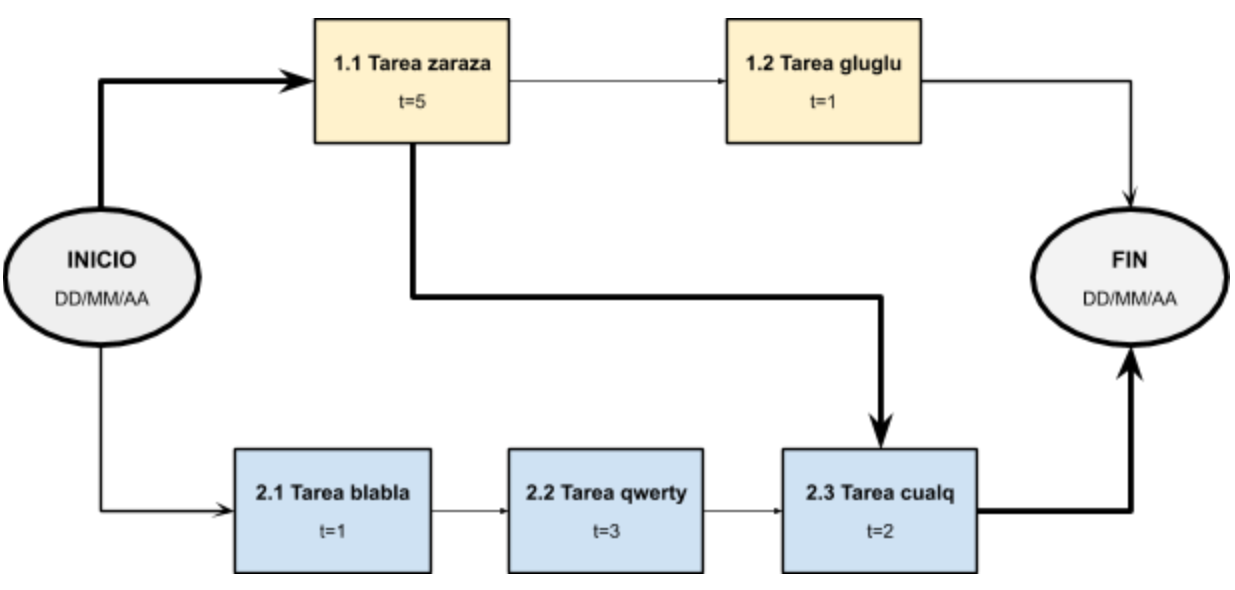
\includegraphics[width=.8\textwidth]{./Figuras/AoN.png}
\caption{Diagrama de \textit{Activity on Node}.}
\label{fig:AoN}
\end{figure}

Indicar claramente en qué unidades están expresados los tiempos.
De ser necesario indicar los caminos semi críticos y analizar sus tiempos mediante un cuadro.
Es recomendable usar colores y un cuadro indicativo describiendo qué representa cada color.




\section{11. Diagrama de Gantt}
\label{sec:gantt}
\textbf{ Supuesto:} se trabaja 3 horas por día, inclusive fines de semana.
\begin{figure}[htpb]
  \begin{center}
    \begin{ganttchart}[
      time slot unit=day,
      time slot format=isodate,
      x unit=0.060cm,
      y unit title=0.6cm,
      y unit chart=0.5cm,
      milestone label font=\scriptsize,
      group label font=\scriptsize,
        bar label font=\tiny,
      milestone/.append style={xscale=4}
      ]{2025-05-1}{2025-12-12}
      \gantttitlecalendar*{2025-05-1}{2025-12-12}{year} \\
      \gantttitlecalendar*{2025-05-1}{2025-12-12}{month} \\

\ganttgroup{Duración Total}{2025-05-1}{2025-12-12} \\

% Fase 1: Análisis y Diseño
\ganttgroup{1. Análisis y Diseño}{2025-05-1}{2025-05-21} \\
\ganttbar{1.1 Requerimientos}{2025-05-1}{2025-05-02} \\
\ganttbar{1.2 Diseño Arquitectura}{2025-05-03}{2025-05-07} \\
\ganttbar{1.3 Evaluación Tecnologías}{2025-05-08}{2025-05-12} \\
\ganttbar{1.4 Diagramas}{2025-05-13}{2025-05-16} \\
\ganttbar{1.5 Validación}{2025-05-17}{2025-05-21} \\
% Fase 2: Aprendizaje
\ganttgroup{2. Aprendizaje}{2025-05-22}{2025-06-08} \\
\ganttbar{2.1 Protocolo MQTT}{2025-05-22}{2025-05-25} \\
\ganttbar{2.2 ESP32-C3}{2025-05-26}{2025-05-29} \\
\ganttbar{2.3 API REST}{2025-05-30}{2025-06-02} \\
\ganttbar{2.4 Interfaz Web}{2025-06-03}{2025-06-06} \\
\ganttbar{2.5 Manejo Errores}{2025-06-07}{2025-06-08} \\
% Fase 3: Desarrollo Firmware
\ganttgroup{3. Desarrollo Firmware}{2025-06-09}{2025-07-08} \\
\ganttbar{3.1 Comunicación RS-232}{2025-06-09}{2025-06-13} \\
\ganttbar{3.2 Cola en RAM}{2025-06-14}{2025-06-18} \\
\ganttbar{3.3 Publicación MQTT}{2025-06-19}{2025-06-25} \\
\ganttbar{3.4 Suscripción MQTT}{2025-06-26}{2025-06-30} \\
\ganttbar{3.5 Manejo Comandos}{2025-07-01}{2025-07-05} \\
\ganttbar{3.6 Reconexión}{2025-07-06}{2025-07-08} \\
% Fase 4: Pruebas y Documentación
\ganttgroup{4. Pruebas y Documentación}{2025-07-09}{2025-07-24} \\
% Fase 5: Desarrollo API REST
\ganttgroup{5. Desarrollo API REST}{2025-07-25}{2025-08-20} \\
\ganttbar{5.1 Modelo BD}{2025-07-25}{2025-07-28} \\
\ganttbar{5.2 Endpoints GET}{2025-07-29}{2025-08-01} \\
\ganttbar{5.3 Procesamiento}{2025-08-02}{2025-08-05} \\
\ganttbar{5.4 Endpoints POST}{2025-08-06}{2025-08-09} \\
\ganttbar{5.5 Integración MQTT}{2025-08-10}{2025-08-13} \\
\ganttbar{5.6 Autenticación}{2025-08-14}{2025-08-17} \\
\ganttbar{5.7 Pruebas API}{2025-08-18}{2025-08-20} \\

\ganttmilestone{Hito 1: Core Funcional}{2025-08-20} \\
% Fase 6: Interfaz Web
\ganttgroup{6. Interfaz Web}{2025-08-26}{2025-09-19} \\
\ganttbar{6.1 Diseño UI}{2025-08-26}{2025-08-30} \\
\ganttbar{6.2 Visualización}{2025-08-31}{2025-09-04} \\
\ganttbar{6.3 Comandos UI}{2025-09-05}{2025-09-09} \\
\ganttbar{6.4 Integración API}{2025-09-10}{2025-09-13} \\
\ganttbar{6.5 Pruebas Usabilidad}{2025-09-14}{2025-09-19} \\
% Fase 7: Pruebas Finales
\ganttgroup{7. Pruebas Finales}{2025-09-20}{2025-10-24} \\
\ganttbar{7.1 Pruebas UI}{2025-09-20}{2025-09-24} \\
\ganttbar{7.2 Configuración Broker}{2025-09-29}{2025-10-02} \\
\ganttbar{7.3 Pruebas Infraestructura}{2025-10-03}{2025-10-06} \\
\ganttbar{7.4 Pruebas Integrales}{2025-10-07}{2025-10-24} \\
% Fase 8: Despliegue
\ganttgroup{8. Despliegue}{2025-10-25}{2025-11-12} \\
\ganttbar{8.1 Implementación}{2025-10-25}{2025-11-12} \\
% Fase 9: Buffer
\ganttgroup{9. Buffer}{2025-11-13}{2025-12-12} \\
\ganttmilestone{Entrega Final}{2025-12-12} \\
\end{ganttchart}

  \end{center}
  \begin{minipage}{\linewidth}
    \caption{\small Diagrama de Gantt.}
  \end{minipage}
  \label{fig:gantt}
\end{figure}

\section{12. Presupuesto detallado del proyecto}
\label{sec:presupuesto}

\begin{consigna}{red}
Si el proyecto es complejo entonces separarlo en partes:
\begin{itemize}
	\item Un total global, indicando el subtotal acumulado por cada una de las áreas.
	\item El desglose detallado del subtotal de cada una de las áreas.
\end{itemize}

IMPORTANTE: No olvidarse de considerar los COSTOS INDIRECTOS.

Incluir la aclaración de si se emplea como moneda el peso argentino (ARS) o si se usa moneda extranjera (USD, EUR, etc). Si es en moneda extranjera se debe indicar la tasa de conversión respecto a la moneda local en una fecha dada.

\end{consigna}

\begin{table}[htpb]
\centering
\begin{tabularx}{\linewidth}{@{}|X|c|r|r|@{}}
\hline
\rowcolor[HTML]{C0C0C0} 
\multicolumn{4}{|c|}{\cellcolor[HTML]{C0C0C0}COSTOS DIRECTOS} \\ \hline
\rowcolor[HTML]{C0C0C0} 
Descripción &
  \multicolumn{1}{c|}{\cellcolor[HTML]{C0C0C0}Cantidad} &
  \multicolumn{1}{c|}{\cellcolor[HTML]{C0C0C0}Valor unitario} &
  \multicolumn{1}{c|}{\cellcolor[HTML]{C0C0C0}Valor total} \\ \hline
 &
  \multicolumn{1}{c|}{} &
  \multicolumn{1}{c|}{} &
  \multicolumn{1}{c|}{} \\ \hline
 &
  \multicolumn{1}{c|}{} &
  \multicolumn{1}{c|}{} &
  \multicolumn{1}{c|}{} \\ \hline
\multicolumn{1}{|l|}{} &
   &
   &
   \\ \hline
\multicolumn{1}{|l|}{} &
   &
   &
   \\ \hline
\multicolumn{3}{|c|}{SUBTOTAL} &
  \multicolumn{1}{c|}{} \\ \hline
\rowcolor[HTML]{C0C0C0} 
\multicolumn{4}{|c|}{\cellcolor[HTML]{C0C0C0}COSTOS INDIRECTOS} \\ \hline
\rowcolor[HTML]{C0C0C0} 
Descripción &
  \multicolumn{1}{c|}{\cellcolor[HTML]{C0C0C0}Cantidad} &
  \multicolumn{1}{c|}{\cellcolor[HTML]{C0C0C0}Valor unitario} &
  \multicolumn{1}{c|}{\cellcolor[HTML]{C0C0C0}Valor total} \\ \hline
\multicolumn{1}{|l|}{} &
   &
   &
   \\ \hline
\multicolumn{1}{|l|}{} &
   &
   &
   \\ \hline
\multicolumn{1}{|l|}{} &
   &
   &
   \\ \hline
\multicolumn{3}{|c|}{SUBTOTAL} &
  \multicolumn{1}{c|}{} \\ \hline
\rowcolor[HTML]{C0C0C0}
\multicolumn{3}{|c|}{TOTAL} &
   \\ \hline
\end{tabularx}%
\end{table}


\section{13. Gestión de riesgos}
\label{sec:riesgos}

\begin{consigna}{red}
a) Identificación de los riesgos (al menos cinco) y estimación de sus consecuencias:
 
Riesgo 1: detallar el riesgo (riesgo es algo que si ocurre altera los planes previstos de forma negativa)
\begin{itemize}
	\item Severidad (S): mientras más severo, más alto es el número (usar números del 1 al 10).\\
	Justificar el motivo por el cual se asigna determinado número de severidad (S).
	\item Probabilidad de ocurrencia (O): mientras más probable, más alto es el número (usar del 1 al 10).\\
	Justificar el motivo por el cual se asigna determinado número de (O). 
\end{itemize}   

Riesgo 2:
\begin{itemize}
	\item Severidad (S): X.\\
	Justificación...
	\item Ocurrencia (O): Y.\\
	Justificación...
\end{itemize}

Riesgo 3:
\begin{itemize}
	\item Severidad (S):  X.\\
	Justificación...
	\item Ocurrencia (O): Y.\\
	Justificación...
\end{itemize}


b) Tabla de gestión de riesgos:      (El RPN se calcula como RPN=SxO)

\begin{table}[htpb]
\centering
\begin{tabularx}{\linewidth}{@{}|X|c|c|c|c|c|c|@{}}
\hline
\rowcolor[HTML]{C0C0C0} 
Riesgo & S & O & RPN & S* & O* & RPN* \\ \hline
       &   &   &     &    &    &      \\ \hline
       &   &   &     &    &    &      \\ \hline
       &   &   &     &    &    &      \\ \hline
       &   &   &     &    &    &      \\ \hline
       &   &   &     &    &    &      \\ \hline
\end{tabularx}%
\end{table}

Criterio adoptado: 

Se tomarán medidas de mitigación en los riesgos cuyos números de RPN sean mayores a...

Nota: los valores marcados con (*) en la tabla corresponden luego de haber aplicado la mitigación.

c) Plan de mitigación de los riesgos que originalmente excedían el RPN máximo establecido:
 
Riesgo 1: plan de mitigación (si por el RPN fuera necesario elaborar un plan de mitigación).
  Nueva asignación de S y O, con su respectiva justificación:
  \begin{itemize}
	\item Severidad (S*): mientras más severo, más alto es el número (usar números del 1 al 10).
          Justificar el motivo por el cual se asigna determinado número de severidad (S).
	\item Probabilidad de ocurrencia (O*): mientras más probable, más alto es el número (usar del 1 al 10).
          Justificar el motivo por el cual se asigna determinado número de (O).
	\end{itemize}

Riesgo 2: plan de mitigación (si por el RPN fuera necesario elaborar un plan de mitigación).
 
Riesgo 3: plan de mitigación (si por el RPN fuera necesario elaborar un plan de mitigación).

\end{consigna}


\section{14. Gestión de la calidad}
\label{sec:calidad}

\begin{consigna}{red}
Elija al menos diez requerimientos que a su criterio sean los más importantes/críticos/que aportan más valor y para cada uno de ellos indique las acciones de verificación y validación que permitan asegurar su cumplimiento.

\begin{itemize} 
\item Req \#1: copiar acá el requerimiento con su correspondiente número.

\begin{itemize}
	\item Verificación para confirmar si se cumplió con lo requerido antes de mostrar el sistema al cliente. Detallar.
	\item Validación con el cliente para confirmar que está de acuerdo en que se cumplió con lo requerido. Detallar. 
\end{itemize}

\end{itemize}

Tener en cuenta que en este contexto se pueden mencionar simulaciones, cálculos, revisión de hojas de datos, consulta con expertos, mediciones, etc.  

Las acciones de verificación suelen considerar al entregable como ``caja blanca'', es decir se conoce en profundidad su funcionamiento interno.  

En cambio, las acciones de validación suelen considerar al entregable como ``caja negra'', es decir, que no se conocen los detalles de su funcionamiento interno.

\end{consigna}

\section{15. Procesos de cierre}    
\label{sec:cierre}

\begin{consigna}{red}
Establecer las pautas de trabajo para realizar una reunión final de evaluación del proyecto, tal que contemple las siguientes actividades:

\begin{itemize}
	\item Pautas de trabajo que se seguirán para analizar si se respetó el Plan de Proyecto original:\\
	 - Indicar quién se ocupará de hacer esto y cuál será el procedimiento a aplicar. 
	\item Identificación de las técnicas y procedimientos útiles e inútiles que se emplearon, los problemas que surgieron y cómo se solucionaron:\\
	 - Indicar quién se ocupará de hacer esto y cuál será el procedimiento para dejar registro.
	\item Indicar quién organizará el acto de agradecimiento a todos los interesados, y en especial al equipo de trabajo y colaboradores:\\
	  - Indicar esto y quién financiará los gastos correspondientes.
\end{itemize}

\end{consigna}

\end{document}
